%
% TTÜ Style Thesis template for LaTeX
%
% Public Version 1.1
% 2019 Adjusted by Frank Korving for his TTÜ Bachelor Thesis, with contributions from Sander Arnus
%
% Public version 1.0
% 2010 - 2013 Thijs Nugteren and Joos Buijs for TU/e Master Thesis
%
% THIS IS THE MAIN FILE (i.e. compile this file, compiling the others directly won't work)
%
\documentclass[12pt, a4paper]{report}

% all the other includes etc. are done in the thesis.sty file.
\usepackage{thesis}
\usepackage{multicol}

%
% These commands need to be defined in order to produce a correct and personalized document
%
\newcommand{\doctitle}{Loogikafunktsioonide süsteem}
\newcommand{\docsubtitle}{Kodutöö 1}

\newcommand{\me}{Arti Zirk}
\newcommand{\studentcode}{176119IDDR}
\newcommand{\university}{TALLINNA TEHNIKAÜLIKOOL}
\newcommand{\school}{INFOTEHNOLOOGIA TEADUSKOND}
\newcommand{\department}{IT SÜSTEEMIDE ARENDUS}

\newcommand{\supervisor}{Main Supervisor Name}
\newcommand{\supervisortitle}{PhD}
\newcommand{\cosupervisor}{Secondary Supervisor Name}
\newcommand{\cosupervisortitle}{MsC}
\newcommand{\keywords}{Important, comma, separated, keywords, applicable, to, your, thesis}
\newcommand{\version}{1.0 version}
\newcommand{\monthYear}{Oktoober 2019}
\newcommand{\Year}{2019}
\newcommand{\signatureDate}{Oktoober 31, 2019}

\author{\me}

%
% PDF settings
%
\hypersetup {
    pdfauthor={\me},
    pdfsubject={\doctitle},
    pdfkeywords={\keywords}
}

\begin{document}
\pagenumbering{roman}
\begin{titlepage}
\headheight = 57pt
\footskip = 5pt
\headsep = 0pt

\centering
\textsc{\begin{Large}
\university\\
\end{Large} }
\school\\
\department\\

\vspace*{7 cm}

\begin{center}

\me \quad \studentcode\\
\begin{Large}
\textsc{\textbf{\doctitle}}\\
\end{Large}
\docsubtitle\\
\end{center}

%\begin{flushright}
%\textbf{Technical Supervisor}\\ \supervisor\\\supervisortitle\\
%\textbf{Academic Supervisor}\\\cosupervisor\\\cosupervisortitle
%\end{flushright}

\vfill

Tallinn \Year
\end{titlepage}

\normalsize

\chapter*{\centerline{Autorideklaratsioon}}\label{chapter:declaration}
\hfill \\
Kinnitan, et olen koostanud antud kodutöö iseseisvalt ning seda ei ole kellegi teise poolt
varem kaitsmisele esitatud. Kõik töö koostamisel kasutatud teiste autorite tööd, olulised
seisukohad, kirjandusallikatest ja mujalt pärinevad andmed on töös viidatud.

\vskip1in
\begin{flushleft}
\begin{tabular}{p{2.0cm}p{6.0cm}p{4.0cm}}
  Autor: & \me  & \\% ......................................\\
  %&& \hfill(signature)\\
  Kuupäev: & \signatureDate &\\
  \\
  \\

% Uncomment the following to add supervisor declaration
%  \multicolumn{3}{l}{The thesis adheres to all specified requirements}\\
%  \hfill \\
%  Supervisor: & \supervisor & ......................................\\
%  && \hfill(signature)\\
%  Date: & \signatureDate &\\


\end{tabular}
\end{flushleft}

%\chapter*{\centerline{Annotatsioon}}\label{chapter:abstract-eesti}
%\input{chapters/abstract-eesti.tex}
\pagebreak

%\chapter*{\centerline{Abstract}}\label{chapter:abstract}
%\input{chapters/abstract}
%\pagebreak

%\chapter*{\centerline{List of abbreviations and terms}}\label{chapter:terms}
%\input{chapters/terms_abbreviations.tex}
%\pagebreak

\phantomsection
\setcounter{tocdepth}{2}    % Sets maximum depth of Table Of Contents
\renewcommand{\contentsname}{Sisukord}
\tableofcontents

%\clearpage \phantomsection
%\setcounter{figure}{0}
%\addcontentsline{toc}{chapter}{\listfigurename}
%\listoffigures

%\clearpage \phantomsection
%\addcontentsline{toc}{chapter}{\listtablename}
%\listoftables

\chapter{Lähteülesande genereerimine}\label{chapter:lähteülesanne}
\setcounter{page}{0}
%from here on, start the 'real' page numbering, from 1, with normal digits
\pagenumbering{arabic}
Loogikaülesanne luuakse matrikli \studentcode{} järgi.

\begin{table}[!ht]
\centering
\begin{tabular}{|l l l|}
 \hline
 fn & ühed & määramatused \\
 \hline
 1: & \tt{20CE0223} & \tt{AEF560B} \\
 2: & \tt{19345B97} & \tt{866C932} \\
 3: & \tt{99B1AD47} & \tt{333B39C2} \\
 4: & \tt{171022C3} & \tt{7B00B96} \\
 \hline
\end{tabular}
\caption{Ühtede ja määramatuste piirkonnad funktsioonides}
\label{table:1}
\end{table}

Tabeli \ref{table:1} abil saadakse järgmine funktsioonide süsteem:
\[\begin{array}{l}
f1(x_1, x_2, x_3, x_4) = \sum(0,2,3,12,14)_1 (5,6,10,11,15)_\_ \\
f2(x_1, x_2, x_3, x_4) = \sum(1,3,4,5,7,9,11)_1 (2,6,8,12)_\_ \\
f3(x_1, x_2, x_3, x_4) = \sum(1,4,7,9,10,11,13)_1 (2,3,12)_\_ \\
f4(x_1, x_2, x_3, x_4) = \sum(0,1,2,3,7,12)_1 (6,9,11)_\_ \\
\end{array}\]
Samaväärne tõeväärtustabel on kuvatud tabelis \ref{table:2}
\begin{table}[ht!]
    \centering
    \begin{tabular}{|c|c c c c|c c c c|}
            \hline
            & \(x_1\)&\(x_2\)&\(x_3\)&\(x_4\) & \(f1\)&\(f2\)&\(f3\)&\(f4\)\\
            \hline
            0 & 0&0&0&0 & 1&0&0&0\\
            1 & 0&0&0&1 & 0&1&1&1\\
            2 & 0&0&1&0 & 1&-&-&1\\
            3 & 0&0&1&1 & 1&1&-&1\\
            \hline
            4 & 0&1&0&0 & 0&1&1&0\\
            5 & 0&1&0&1 & -&1&0&0\\
            6 & 0&1&1&0 & -&-&0&-\\
            7 & 0&1&1&1 & 0&1&1&1\\
            \hline
            8 & 1&0&0&0 & 0&-&0&0\\
            9 & 1&0&0&1 & 0&1&1&-\\
            A & 1&0&1&0 & -&0&1&0\\
            B & 1&0&1&1 & -&1&1&-\\
            \hline
            C & 1&1&0&0 & 1&-&-&1\\
            D & 1&1&0&1 & 0&0&1&0\\
            E & 1&1&1&0 & 1&0&0&0\\
            F & 1&1&1&1 & -&0&0&0\\
            \hline
    \end{tabular}
    \caption{Funktsioonide süsteem tõeväärtustabeli kujul}
    \label{table:2}
\end{table}{}

\chapter{Minimeerimine}\label{chapter:minimeerimine}
Minimeerimine on tehtud programmi \verb|espresso|\footnote{\url{https://github.com/classabbyamp/espresso-logic}} abil. Sisendiks on tabelis \ref{table:2} toodud tõeväärtus tabel.
Argumendi \verb|-Dopoall| kasutamisel olen välja valinud kaks huvitavamat lahendust erinevate faasidega.

Kodutöö ülesande kirjelduses on öeldud, et tuleks optimeerida pindala ning kiirust. Lisaks on piiratud, et loogika elementidel saab olla kuni 3 sisendit.
Ehk siis \verb|espresso| \verb|-Dopoall| väljundis on tähtis jälgida implikantide arvu (c) ning sisendite ja väljundite koguarvu (tot).

\begin{lstlisting}[
    basicstyle=\ttfamily\footnotesize,
    caption=-Dopoall faas 0000,
]
# phase is ---- 0000
# ESPRESSO  	Time was 0.00 sec, cost is c=9(0) in=26 out=16 tot=42
\end{lstlisting}

Faasi 0000 implikantide arv on c=9, teiste faaside korral on see arv suurem.

Kogu \verb|espresso -Dopoall| leiab lisade all olevast listingust nr\ref{espresso:dopoall}.

\begin{lstlisting}[
    basicstyle=\ttfamily\footnotesize,
    caption=-o eqntott faas 0000,
]
y1 = (!x3&x4) | (!x1&x2) | (x1&!x2&!x4);
y2 = (!x2&!x3&!x4) | (x1&x2&x4) | (x1&!x2&!x4) | (x1&x2&x3);
y3 = (x2&x3&!x4) | (!x1&x2&!x3&x4) | (!x2&!x3&!x4) | (x1&x2&x3);
y4 = (!x1&x2&!x3&x4) | (!x1&!x3&!x4) | (x1&x2&x4) | (x1&!x2&!x4) |
     (x1&x2&x3);
\end{lstlisting}

Kui vaadata \verb|-eqntott| argumendi väljundit faaasi 0000 korral siis on näha, et meil tekib väga palju üle 3 sisendiga loogika elemente. Faasi 0000 valimine edasiseks optimeerimiseks ei oleks mõtekas.

\begin{lstlisting}[
    basicstyle=\ttfamily\footnotesize,
    caption=-Dopoall faas 0101,
]
# phase is ---- 0101
# ESPRESSO  	Time was 0.00 sec, cost is c=10(0) in=27 out=12 tot=39
\end{lstlisting}

Faasi 0101 korral on näha, et implikante on ühe võrra rohkem kuid kogu sisendite ja väljundite arv tot=39 mis on võrreldes teiste faasidega kõige väiksem.

\begin{lstlisting}[
    basicstyle=\ttfamily\footnotesize,
    caption=-o eqntott faas 0101,
]
y1 = (x1&!x2) | (!x3&x4) | (!x1&x2);
y2 = (!x2&x4) | (!x1&x2);
y3 = (!x1&x2&!x3&x4) | (!x1&x3&!x4) | (x1&x2&x3) | (!x2&!x3&!x4);
y4 = (x1&x2&!x3&!x4) | (!x1&x3) | (!x2&x4);
\end{lstlisting}

Vaadates \verb|-eqntott| argumendiga saadud tulemust näeme, et üle 3 sisendiga loogika elemente on siin ka üsna vähe.

Edasiseks optimeerimiseks võtame aluseks faasi 0101.

\chapter{Minimeerimine}\label{chapter:loogikaskeem}
\section{Esialgne funktsioonide süsteemi skeem}
Kirjutatakse välja esialgne skeem ilma elementide sisendite piiranguta ning see järel
natuke lahti kirjutades vastavalt ülesande 3 sisendiga loogikaelementide piirangule.

\newcommand\bnot[1]{\mathop{\overline{#1}}}
\newcommand\nand[0]{\bnot{\wedge}}
\newcommand\nor[0]{\bnot{\vee}}

\begin{multicols}{2}
\(\begin{array}{l}
t_1 = x_1 \bnot{x_2} \\
t_2 = \bnot{x_3 } x_4 \\
t_3 = \bnot{x_1} x_2 \\
t_4 = \bnot{x_2} x_4 \\
t_5 = \bnot{x_1} x_2 \\
t_6 = \bnot{x_1} x_2 \bnot{x_3} x_4 \\
t_7 = \bnot{x_1} x_3 \bnot{x_4} \\ 
t_8 = x_1 x_2 x_3 \\
t_9 = \bnot{x_2} \bnot{x_3} \bnot{x_4} \\
t_{10} = x_1 x_2 \bnot{x_3} \bnot{x_4} \\
t_{11} = \bnot{x_1} x_3 \\
t_{12} = \bnot{x_2} x_4 \\
y_1 = \bnot{t_1 | t_2 | t_3} \\
y_2 = t_4 | t_5 \\ 
y_3 = \bnot{t_6 | t_7 | t_8 | t_9} \\
y_4 = t_{10} | t_{11} | t_{12} \\
\end{array}\)

\columnbreak

\(\begin{array}{l r}
t_1 = x_1 \bnot{x_2} \\
t_2 = \bnot{x_3} x_4 \\
t_3 = \bnot{x_1} x_2 & [=t_5]\\
t_4 = \bnot{x_2} x_4 \\
t_5 = \bnot{x_1} x_2 & [=t_3]\\
{\color{red}t_{61} = \bnot{x_1} \bnot{x_3}} \\
t_6 = {\color{red}t_{61}} x_2 x_4 \\
t_7 = \bnot{x_1} x_3 \bnot{x_4} \\ 
t_8 = x_1 x_2 x_3 & [= {\color{red}t_{101}} x_3]\\
t_9 = \bnot{x_2} \bnot{x_3} \bnot{x_4} \\
{\color{red}t_{101} = x_1 x_2} \\
t_{10} = {\color{red}t_{101}} \bnot{x_3} \bnot{x_4} \\
t_{11} = \bnot{x_1} x_3 \\
t_{12} = \bnot{x_2} x_4 \\
y_1 = \bnot{t_1 | t_2 | t_3} \\
y_2 = t_4 | t_5 \\ 
{\color{red}y_{31} = t_6 | t_7} \\
y_3 = \bnot{{\color{red}y_{31}} | t_8 | t_9} \\
y_4 = t_{10} | t_{11} | t_{12} \\
\end{array}\)
\end{multicols}

\section{Pindala ja viite analüüs}
Järgmisena analüüsitakse loogikafunktsioonide süsteemi pindala ja viidet.
Viite parameetrid on võetud koduse ülesande lehelt ning on toodud
tabelis \ref{table:logic_elements}.

\begin{table}
\centering
\begin{tabular}{|c|c|c|}
\hline
Element & Suurus & Viide \\
\hline
2-NAND & 1.0 & 1.0 \\
\hline
bnot & 1.5 & 1.5 \\ 
2-NOR & 1.5 & 1.5 \\
3-NAND & 1.5 & 1.5 \\
\hline
2-OR & 2.0 & 2.0 \\
2-AND & 2.0 & 2.0 \\
2-XOR & 2.0 & 2.0 \\
3-NOR & 2.0 & 2.0 \\
\hline
3-OR & 2.5 & 2.5 \\
3-AND & 2.5 & 2.5 \\
3-XOR & 2.5 & 2.5 \\
\hline
\end{tabular}
\caption{Loogika elementide suurused ja viited}
\label{table:logic_elements}
\end{table}

\pagebreak

Implikantide järel on välja toodud realiseeritava loogika elemendi pindala/viide ning kogu viide.

\(\begin{array}{l r r}
x_{1i} = \bnot{x_1} & [1.5/1.5] & 1.5\\
x_{2i} = \bnot{x_2} & [1.5/1.5] & 1.5 \\
x_{3i} = \bnot{x_3} & [1.5/1.5] & 1.5 \\
x_{4i} = \bnot{x_4} & [1.5/1.5] & 1.5 \\

c_1 = x_{1i} x_2  & [2.0/2.0] & 1.5+2.0=3.5\\
c_2 = x_1 x_2 & [2.0/2.0] & 2.0\\ 

t_1 = x_1 x_{2i} & [2.0/2.0] & 1.5+2.0=3.5\\
t_2 = x_{3i} x_4 & [2.0/2.0] & 1.5+2.0=3.5\\
t_4 = x_{2i} x_4 & [2.0/2.0] & 1.5+2.0=3.5\\
t_{61} = x_{1i} x_{3i} & [2.0/2.0] & 1.5+2.0=3.5\\
t_6 = t_{61} x_2 x_4 & [2.5/2.5] & 3.5+2.5=6.0\\
t_7 = x_{1i} x_3 x_{4i} & [2.5/2.5] & 1.5+2.5=3.5\\ 
t_8 = c_2 x_3 & [2.0/2.0] & 2.0+2.0=4.0\\
t_9 = x_{2i} x_{3i} x_{4i} & [2.5/2.5] & 1.5+2.5=3.5 \\
t_{10} = c_2 x_{3i} x_{4i} & [2.5/2.5] & 2.0+2.5=4.5\\
t_{11} = x_{1i} x_3 & [2.0/2.0] & 1.5+2.0=3.5\\
t_{12} = x_{2i} x_4 & [2.0/2.0] & 1.5+2.0=3.5 \\
%\end{array}\)
%\(\begin{array}{l r r}
y_{1i} = t_1 | t_2 | c_1 & [2.5/2.5] & 3.5+2.5=6.0 \\
y_1 = \bnot{y_{1i}} & [1.5/1.5] & 6.0+1.5=7.5 \\
y_2 = t_4 | c_1 & [2.0/2.0] & 3.5+2.0=5.5\\ 
y_{31} = t_6 | t_7 & [2.0/2.0] & 6.0+2.0=8.0\\
y_{3i} = y_{31} | t_8 | t_9 & [2.5/2.5] & 8.0+2.5=10.5 \\
y_3 = \bnot{y_{3i}} & [1.5/1.5] & 10.5+1.5=12.0\\
y_4 = t_{10} | t_{11} | t_{12} & [2.5/2.5] & 4.5+2.5=7.0\\
\end{array}\)

Elemendid: 6 x NOT, 9 x 2-AND, 4 x 3-AND, 2 x 2-OR, 3 x 3-OR.

Kokku: 24 elementi, suurus 46, kriitiline tee 12.

\section{Ühiste alamavaldiste otsimine}

\(\begin{array}{l r}
y_1 = (x_1 \bnot{x_2}) | (\bnot{x_3} x_4) | (\bnot{x_1} x_2)\\
/(\bnot{x_3} x_4) \rightarrow (x_1 \bnot{x_2}) |  (\bnot{x_1} x_2) & = x_1  \oplus  x_2 \\ 
\end{array}\)

\(\begin{array}{l r}
y_2 = (\bnot{x_2} x_4) | (\bnot{x_1} x_ 2)
\end{array}\)

\(\begin{array}{l r}
y_3 = (\bnot{x_1} x_2 \bnot{x_3} x_4) | (\bnot{x_1} x_3 \bnot{x_4}) |
    (x_1 x_2 x_3) | (\bnot{x_2} \bnot{x_3} \bnot{x_4}) \\
/\bnot{x_1} \rightarrow (x_2 \bnot{x_3} x_4) | (x_3 \bnot{x_4}) \\
/x_2 \rightarrow (\bnot{x_1} \bnot{x_3} x_4) | (x_1 x_3) \\
/\bnot{x_2} \rightarrow (\bnot{x_3} \bnot{x_4}) & (\bnot{x_3} \bnot{x_4}) = c_1 \\
/x_3 \rightarrow (\bnot{x_1} \bnot{x_4}) | (x_1 x_2) & (x_1 x_2) = c_2\\
/\bnot{x_3} \rightarrow (\bnot{x_1} x_2 x_4) | (\bnot{x_2} \bnot{x_4})\\
/\bnot{x_4} \rightarrow (\bnot{x_1} x_3) | (\bnot{x_2} \bnot{x_3})

\end{array}\)

\(\begin{array}{l r}
y_4 = (x_1 x_2 \bnot{x_3} \bnot{x_4}) | (\bnot{x_1} x_3) | (\bnot{x_2} x_4) \\
/(x_1 x_2) \rightarrow (\bnot{x_3} \bnot{x_4}) & = c_1 \\
/(\bnot{x_3} \bnot{x_4}) \rightarrow (x_1 x_2) & = c_2 \\
\end{array}\)

Suur enamus optimeeringuid on leitud intuitiivselt ning pole siin eraldi välja toodud.

\section{Optimeeritud pindala ja viite analüüs}

\(\begin{array}{l r r}
x_{1i} = \bnot{x_1} & [1.5/1.5] & 1.5\\
x_{2i} = \bnot{x_2} & [1.5/1.5] & 1.5 \\
x_{3i} = \bnot{x_3} & [1.5/1.5] & 1.5 \\
x_{4i} = \bnot{x_4} & [1.5/1.5] & 1.5 \\
\\
c_1 = x_1 x_2 & [2.0/2.0] & 2.0\\ 
\\
t_1 = x_1  \oplus  x_2 & [2.0/2.0] & 2.0\\
t_2 = x_{3i} \nand x_4 & [1.0/1.0] & 1.5+1.0=2.5\\
y_1 =  t_1  t_2 & [2.0/2.0] & 2.5+2.0=4.5 \\
\\
t_3 = x_{2i} \nand x_4 & [1.0/1.0] & 1.5+1.0=2.5\\
t_4 = x_{1i} \nand x_2 & [1.0/1.0] & 1.5+1.0=2.5\\
y_2 = t_3 \nand t_4 & [1.0/1.0] & 2.5+2.0=4.5 \\
\\
t_{51} = x_1 \oplus x_3 & [2.0/2.0] & 2.0\\
t_{52} = x_2 x_4 & [2.0/2.0] & 2.0\\
t_5 = t_{51} \nand t_{52} & [1.0/1.0] & 2.0+1.0=3.0\\
t_{61} = x_1 \nor x_4 & [1.5/1.5] & 1.5\\
t_6 = t_{61} \nand x_3 & [1.0/1.0] & 1.5+1.0=2.5 \\
t_7 = c_1 \nand x_3 & [1.0/1.0] & 2.0+1.0=3.0\\
t_8 = x_2 | x_3 | x_4 & [2.5/2.5] & 2.5\\
y_{31} = t_7  t_8 & [2.0/2.0] & 3.0+2.0 = 5.0\\
y_3 = t_5 t_6 y_{31} & [2.0/2.0] & 5.0+2.0=7.0\\
\\
t_9 = x_3 \nor x_4 & [1.5/1.5] & 1.5\\
t_{10} = c_1 \nand t_9 & [2.0/2.0] & 2.0+2.0=4.0 \\
t_{11} = x_{1i} \nand x_3 & [1.0/1.0] & 1.5+1.0=2.5 \\
t_{12} = x_{2i} \nand x_4 & [1.0/1.0] & 1.5+1.0=2.5\\ 
y_{4i} = t_{10}  t_{11}  t_{12} & [2.5/2.5] & 4.0+2.5=6.5 \\
y_4 = \bnot{y_{4i}} & [1.5/1.5] & 6.5+1.5=8.0\\
\end{array}\)

Elemendid: 5 x NOT, 4 x 2-AND, 2 x 3-AND, 1 x 3-OR, 10 x 2-NAND, 

Kokku: 22 (-2) elementi, suurus 33 (-13), kriitiline tee 8 (-4).

Optimeeritud loogikasüsteemil on väiksem pindala, väiksem voolu tarve ning on kiirem.

\chapter{Modeleerimine}\label{chapter:modeleerimine}
Modeleerimiseks on kasutatud \verb|ghdl| ning \verb|gtkwave| rakendusi. VHDL koodi aluseks on kodutöö näidis projekti kood.

\begin{figure}[ht]
    \centering
    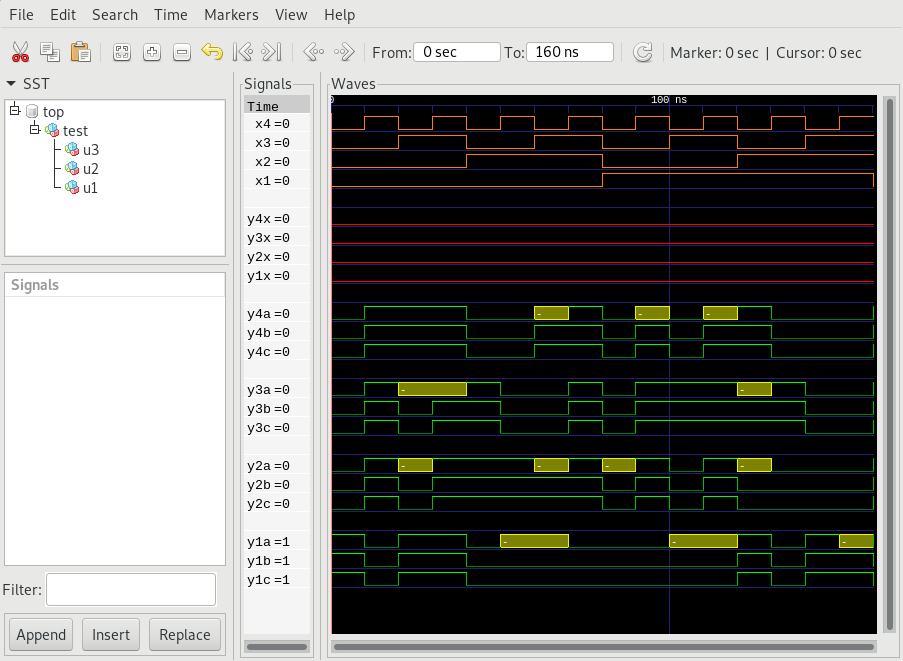
\includegraphics[width=1\textwidth]{figures/overview.png}
    \caption{\textit{Testpingi väljund}}
    \label{fig:wave_overview}
\end{figure}

Joonisel \ref{fig:wave_overview}, \(x_1, x_2, x_3, x_4\) on testpingi sisendid, \(y_1x, y_2x, y_3x, y_4x\) on testpingi väljundid ja signaalid \(y\{_1,_2,_3,_4\}\{a,b,c\}\) on tabeli, espresso ja optimeeritud loogikaskeemi väljundid.

\begin{figure}[ht]
    \centering
    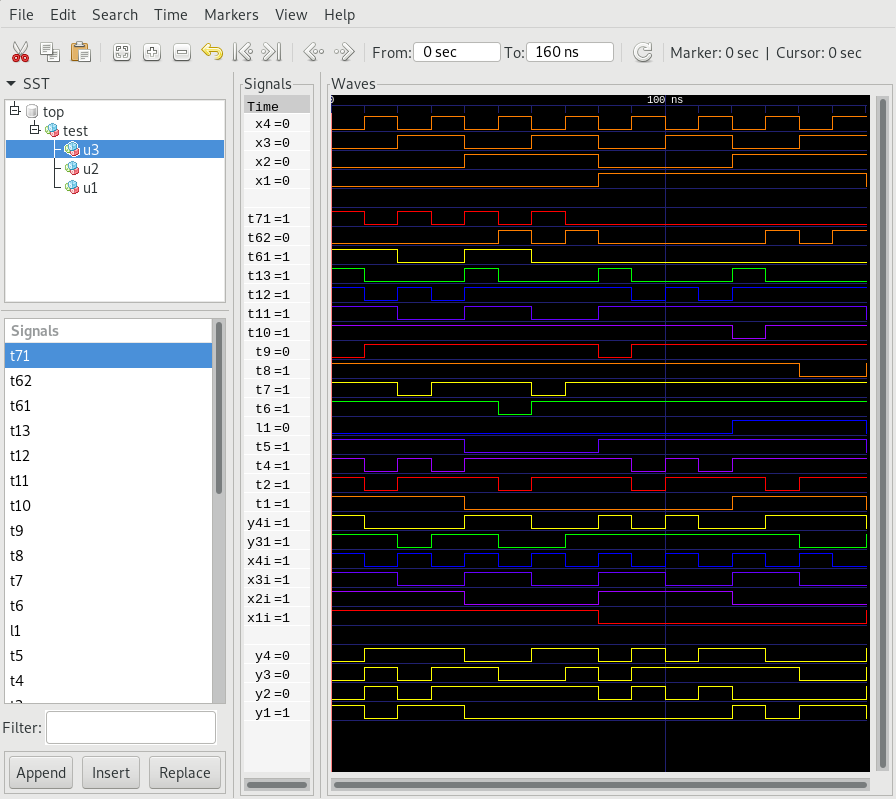
\includegraphics[width=1\textwidth]{figures/opti1.png}
    \caption{\textit{Optimeeritud loogikaskeemi sisemised väärtused}}
    \label{fig:wave_opti1}
\end{figure}

Joonis \ref{fig:wave_opti1} kuvatud signaalid vastavad lisas toodud \verb|opt1o.vhdl| koodile mille listing nr\ref{fs1opt10} leiab lisadest. Joonis \ref{fig:wave_opti1} kuvatud signaalid vastavad lisas toodud \verb|opt1o.vhdl| koodile mille listing nr\ref{fs1opt10} leiab lisadest. 



%\chapter{Introduction}\label{chapter:introduction}
%\input{chapters/introduction}

%\chapter{First Chapter}\label{chapter:first_chapter}
%\input{chapters/first_chapter.tex}

%\chapter{Second Chapter}\label{chapter:second_chapter}
%\input{chapters/second_chapter.tex}

%\chapter{Summary}\label{chapter:summary} 
%\input{chapters/summary.tex}

%\pagebreak
%\phantomsection
%\addcontentsline{toc}{chapter}{Bibliography}
%\printbibliography

\pagebreak
\phantomsection
\appendix
\addcontentsline{toc}{chapter}{Lisad}
\chapter*{Lisad}
\renewcommand{\thechapter}{\arabic{chapter}}

\addcontentsline{toc}{chapter}{Lisa 1 - espresso -Dopoall}
\label{appendix:espresso:dopoall}
{\let\clearpage\relax\chapter*{Lisa 1 - espresso -Dopoall}}
\begin{lstlisting}[
    basicstyle=\ttfamily\footnotesize,
    caption=Programmi espresso -Dopoall väljund,
    label=espresso:dopoall
]
.i 4
.o 4
0000 1000
0001 0111
0010 1--1
0011 11-1
0100 0110
0101 -100
0110 --0-
0111 0111
1000 0-00
1001 011-
1010 -010
1011 -11-
1100 1--1
1101 0010
1110 1000
1111 -000
.e
# phase is ---- 0000
# ESPRESSO  	Time was 0.00 sec, cost is c=9(0) in=26 out=16 tot=42
# phase is ---- 0001
# ESPRESSO  	Time was 0.00 sec, cost is c=10(0) in=30 out=15 tot=45
# phase is ---- 0010
# ESPRESSO  	Time was 0.00 sec, cost is c=10(0) in=30 out=18 tot=48
# phase is ---- 0011
# ESPRESSO  	Time was 0.00 sec, cost is c=10(0) in=28 out=15 tot=43
# phase is ---- 0100
# ESPRESSO  	Time was 0.00 sec, cost is c=10(0) in=26 out=15 tot=41
# phase is ---- 0101
# ESPRESSO  	Time was 0.00 sec, cost is c=10(0) in=27 out=12 tot=39
# phase is ---- 0110
# ESPRESSO  	Time was 0.00 sec, cost is c=10(0) in=27 out=17 tot=44
# phase is ---- 0111
# ESPRESSO  	Time was 0.00 sec, cost is c=10(0) in=26 out=14 tot=40
# phase is ---- 1000
# ESPRESSO  	Time was 0.00 sec, cost is c=10(0) in=30 out=15 tot=45
# phase is ---- 1001
# ESPRESSO  	Time was 0.00 sec, cost is c=11(0) in=30 out=14 tot=44
# phase is ---- 1010
# ESPRESSO  	Time was 0.00 sec, cost is c=11(0) in=31 out=16 tot=47
# phase is ---- 1011
# ESPRESSO  	Time was 0.00 sec, cost is c=10(0) in=26 out=15 tot=41
# phase is ---- 1100
# ESPRESSO  	Time was 0.00 sec, cost is c=12(0) in=32 out=14 tot=46
# phase is ---- 1101
# ESPRESSO  	Time was 0.00 sec, cost is c=10(0) in=28 out=13 tot=41
# phase is ---- 1110
# ESPRESSO  	Time was 0.00 sec, cost is c=10(0) in=27 out=15 tot=42
# phase is ---- 1111
# ESPRESSO  	Time was 0.00 sec, cost is c=10(0) in=26 out=15 tot=41
\end{lstlisting}

\addcontentsline{toc}{chapter}{Lisa 2 - VHDL kood}
\label{appendix:vhdl}
{\let\clearpage\relax\chapter*{Lisa 1 - VHDL kood}}
\begin{lstlisting}[
    basicstyle=\ttfamily\footnotesize,
    caption=f\_system.vhd
]
library IEEE; use IEEE.std_logic_1164.all;
entity f_system is
  port ( x1, x2, x3, x4: in std_logic;
         y1, y2, y3, y4: out std_logic );
end entity f_system;
\end{lstlisting}

\begin{lstlisting}[
    basicstyle=\ttfamily\footnotesize,
    caption=fs1\_table.vhd
]
-------------------------------------
-- IAY0150 - Homework #1. Truth table
-------------------------------------
-- (C) Arti Zirk - 2019 - Tallinn
-------------------------------------

library IEEE; use IEEE.std_logic_1164.all;
architecture tabel of f_system is
begin
  process (x1, x2, x3, x4)
    variable in_word, out_word: std_logic_vector (3 downto 0);
  begin
    in_word := x1 & x2 & x3 & x4;
    case  in_word  is
      when "0000" => out_word := "1000";
      when "0001" => out_word := "0111";
      when "0010" => out_word := "1--1";
      when "0011" => out_word := "11-1";
      when "0100" => out_word := "0110";
      when "0101" => out_word := "-100";
      when "0110" => out_word := "--0-";
      when "0111" => out_word := "0111";
      when "1000" => out_word := "0-00";
      when "1001" => out_word := "011-";
      when "1010" => out_word := "-010";
      when "1011" => out_word := "-11-";
      when "1100" => out_word := "1--1";
      when "1101" => out_word := "0010";
      when "1110" => out_word := "1000";
      when "1111" => out_word := "-000";
      when others => out_word := "----";
    end case;
    y1 <= out_word(3);    y2 <= out_word(2);
    y3 <= out_word(1);    y4 <= out_word(0);
  end process;
end architecture tabel;
\end{lstlisting}

\begin{lstlisting}[
    basicstyle=\ttfamily\footnotesize,
    caption=fs1\_espr.vhd
]
-----------------------------------------
-- IAY0150 - Homework #1. Espresso result
-----------------------------------------
-- (C) Arti Zirk - 2019 - Tallinn
-----------------------------------------

library IEEE; use IEEE.std_logic_1164.all;
architecture espresso of f_system is
begin
  y1 <= not ((x1 and not x2) or (not x3 and x4) or
        (not x1 and x2));

  y2 <= (not x2 and x4) or  (not x1 and x2);

  y3 <= not ((not x1 and x2 and not x3 and x4) or 
       (not x1 and x3 and not x4) or
       (x1 and x2 and x3) or
       (not x2 and not x3 and not x4));

  y4 <= (x1 and x2 and not x3 and not x4) or
        (not x1 and x3) or (not x2 and x4);
end architecture espresso;
\end{lstlisting}

\begin{lstlisting}[
    basicstyle=\ttfamily\footnotesize,
    caption=fs1\_opt1o.vhd,
    label=fs1opt10
]
-----------------------------------------
-- IAY0150 - Homework #1.
-----------------------------------------
-- (C) Arti Zirk - 2019 - Tallinn
-----------------------------------------

library IEEE; use IEEE.std_logic_1164.all;
architecture opti1 of f_system is
  signal x1i, x2i, x3i, x4i, y31, y4i, t1: std_logic;
  signal t6, t7, t8, t9, t10, t11, t12: std_logic;
  signal t2, t3, t4, t5, l1, t13, t61, t62, t71: std_logic;
begin
  x1i <= not x1;
  x2i <= not x2;
  x3i <= not x3;
  x4i <= not x4;

  l1 <= x1 and x2;

  t1 <= not (x1 xor x2);
  t2 <= x3i nand x4;
  y1 <= t1 and t2;

  t4 <= x2i nand x4;
  t5 <= x1i nand x2;
  y2 <= t4 nand t5;

  t61 <= x1 nor x3;
  t62 <= x2 and x4;
  t6  <= t61 nand t62;
  t71 <= x1 nor x4;
  t7 <= t71 nand x3;
  t8 <= l1 nand x3;
  t9 <= x2 or x3 or x4;
  y31 <= t6 and t7 and t8;
  y3 <= y31 and t9;

  t13 <= x3 nor x4;
  t10 <= l1 nand t13;
  t11 <= x1i nand x3;
  t12 <= x2i nand x4;
  y4i <= t10 and t11 and t12;
  y4 <= not y4i;
end architecture opti1;
\end{lstlisting}


\begin{lstlisting}[
    basicstyle=\ttfamily\footnotesize,
    caption=fs1\_test.vhd
]
------------------------------------------------------------------------
-- IAY0150 - Homework #1. Test bench for the example task.
------------------------------------------------------------------------
-- (C) Peeter Ellervee - 2016 - Tallinn
------------------------------------------------------------------------
library IEEE; use IEEE.std_logic_1164.all;
entity test is
end entity test;

library IEEE; use IEEE.std_logic_1164.all;
architecture bench of test is
  signal x1, x2, x3, x4: std_logic;
  signal y1a, y1b, y1c, y2a, y2b, y2c: std_logic;
  signal y3a, y3b, y3c, y4a, y4b, y4c: std_logic;
  signal y1x, y2x, y3x, y4x: std_logic;
  component f_system
    port ( x1, x2, x3, x4: in std_logic;
           y1, y2, y3, y4: out std_logic );
  end component;
  for U1: f_system use entity work.f_system(tabel);
  for U2: f_system use entity work.f_system(espresso);
  for U3: f_system use entity work.f_system(opti1);

  function compare_signals (s1, s2, s3: std_logic) return std_logic is
  begin
    if  s1='-'  then
      if  s2/=s3  then  return 'X';  end if;
    else
      if  s1/=s2 or s1/=s3  then  return 'X';  end if;
    end if;
    return '0';
  end function compare_signals;
begin
  -- Input signals (after every 10 ns)
  x1 <= '0' after 0 ns, '1' after 80 ns, '0' after 160 ns;
  x2 <= '0' after 0 ns, '1' after 40 ns, '0' after 80 ns, '1' after 120 ns;
  x3 <= '0' after 0 ns, '1' after 20 ns, '0' after 40 ns, '1' after 60 ns,
        '0' after 80 ns, '1' after 100 ns, '0' after 120 ns, '1' after 140 ns;
  x4 <= '0' after 0 ns, '1' after 10 ns, '0' after 20 ns, '1' after 30 ns,
        '0' after 40 ns, '1' after 50 ns, '0' after 60 ns, '1' after 70 ns,
        '0' after 80 ns, '1' after 90 ns, '0' after 100 ns, '1' after 110 ns,
        '0' after 120 ns, '1' after 130 ns, '0' after 140 ns, '1' after 150 ns;

  -- System of Boolean functions
  U1: f_system port map (x1, x2, x3, x4, y1a, y2a, y3a, y4a);
  U2: f_system port map (x1, x2, x3, x4, y1b, y2b, y3b, y4b);
  U3: f_system port map (x1, x2, x3, x4, y1c, y2c, y3c, y4c);
  --y1c<=y1b;  y2c<=y2b;  y3c<=y3b;  y4c<=y4b;
  y1x <= compare_signals (y1a, y1b, y1c);
  y2x <= compare_signals (y2a, y2b, y2c);
  y3x <= compare_signals (y3a, y3b, y3c);
  y4x <= compare_signals (y4a, y4b, y4c);
end architecture bench;
\end{lstlisting}


\begin{lstlisting}[
    basicstyle=\ttfamily\footnotesize,
    caption=make.sh
]
#!/bin/bash
set -x -e

# uses ghdl-mcode variant
# import vhd files
ghdl -i -g *.vhd
# make unit
ghdl -m test
# run unit and export logic graph
ghdl -r test --wave=test.ghw --stop-time=200ns

# send signal to gtkwave to reload open file
gsettings set com.geda.gtkwave reload 0
\end{lstlisting}

%\clearpage
%\phantomsection
%\addcontentsline{toc}{chapter}{Lisa 2 - Something Else}
%\label{chapter:appendix-something-else}
%\chapter*{Appendix 2 - Something Else}
%\textbf{Pythagorean theorem}
\begin{equation}
x^n + y^n = z^n
\end{equation}

\textbf{Normal distribution}%
\begin{equation}
P(x) = \frac{1}{{\sigma \sqrt {2\pi } }}e^{{{ - \left( {x - \mu } \right)^2 } \mathord{\left/ {\vphantom {{ - \left( {x - \mu } \right)^2 } {2\sigma ^2 }}} \right. \kern-\nulldelimiterspace} {2\sigma ^2 }}}
\end{equation}

\end{document}